\chapter{Introducción específica} % Main chapter title

\label{Chapter2} % Change X to a consecutive number; for referencing this chapter elsewhere, use \ref{ChapterX}

%----------------------------------------------------------------------------------------
Este capítulo expone una descripción detallada del sistema, del hardware utilizado y las herramientas de  software necesarias en el desarrollo del trabajo. Se abarcan la descripción del sistema y sus componentes, los \textit{frameworks} y modelos utilizados para detección facial y las herramientas utilizadas en la web.

%----------------------------------------------------------------------------------------
\section{Funcionamiento general del sistema}
El sistema desarrollado en este trabajo consta de varios componentes de hardware que interconectados entre sí son capaces de cubrir todos los requerimientos funcionales planteados en el capítulo \ref{Chapter1}. En la figura \ref{fig:sys_blocks} se muestra el diagrama en bloques del sistema.

\begin{figure}[h]
	\centering
	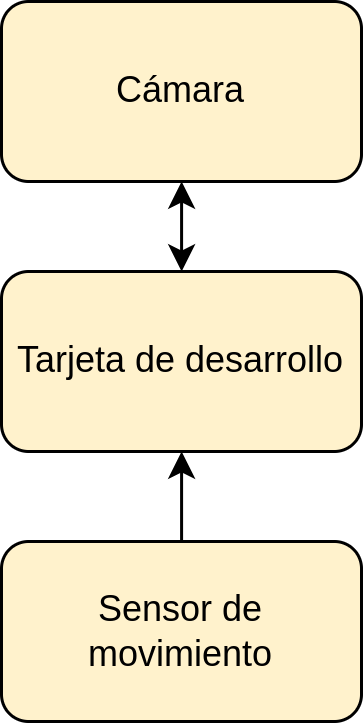
\includegraphics[scale=0.25]{./Figures/sys_blocks.png}
	\caption{Diagrama en bloques del sistema.}
	\label{fig:sys_blocks}
\end{figure}

En el sistema de la figura \ref{fig:sys_blocks}, cuando el sensor de movimiento detecta el movimiento de una persona genera una señal que notifica a la tarjeta de desarrollo sobre este evento. Entonces la tarjeta de desarrollo activa la cámara y obtiene una fotografía para procesarla. La imagen digital obtenida es procesada y utilizada como entrada para los modelos de DL. Cuando se obtienen las inferencias deseadas de los modelos, los resultados son procesados para transmitirlos hacia los servidores en la nube encargados de procesarlos y mostrarlos a los usuarios finales.

\subsection{Tarjeta de desarrollo}
El componente central del sistema es la tarjeta de desarrollo ESP32-S3-DevKitC-1-N8R8 de la empresa Espressif. Tiene como componente central el módulo ESP32-S3-WROOM-1-N8R8 y varios otros componentes que simplifican el proceso de desarrollo de aplicaciones para IoT. En la figura \ref{fig:devkit_comp} se observa una fotografía de la tarjeta con el detalle de sus componentes.

\begin{figure}[h]
	\centering
	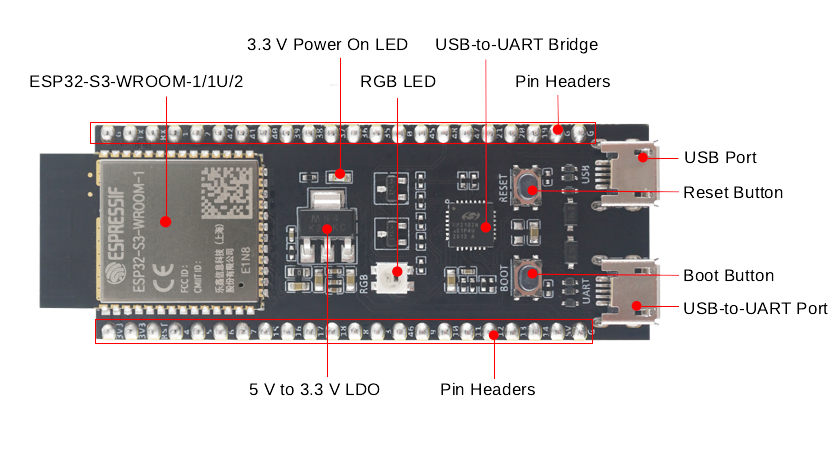
\includegraphics[scale=0.45]{./Figures/devkit_comp.png}
	\caption{Componentes del ESP32-S3-DevKitC-1\protect\footnotemark.}
	\label{fig:devkit_comp}
\end{figure}
\footnotetext{Imagen tomada de: \url{https://docs.espressif.com/projects/esp-idf/en/latest/esp32s3/hw-reference/esp32s3/user-guide-devkitc-1.html}}

El módulo ESP32-S3-WROOM-1-N8R8 es un potente módulo MCU (\textit{Microcontroller Unit}, Unidad de Microcontrolador) de doble núcleo que incorpora Wi-Fi y BLE (\textit{Bluetooth Low Energy}, Bluetooth de Baja Energía) y tiene un amplio conjunto de periféricos. Sus especificaciones técnicas más relevantes se detallan en la tabla \ref{tab:devkit_specs}.

\begin{table}[h]
	\centering
	\caption[ESP32-S3-DevKitC-1 especificaciones]{Tabla de especificaciones del ESP32-S3-DevKitC-1 \cite{devkit_info}}
	\begin{tabular}{lc}   
		\toprule
		\textbf{Característica} 	 & \textbf{Descripción}  \\
		\midrule
		SoC embebido & ESP32-S3R8 \\
		Procesador & Xtensa LX7 doble núcleo de 32 bits \\
		Frecuencia & Hasta 240 MHz \\
		ROM & 384 KB \\
		SRAM & 512 KB \\
		Pines & 41 \\
		Flash & 8 MB \\
		PSRAM & 8 MB \\
		Tipo de antena & PCB \\
		Wi-Fi & 802.11 b/g/n hasta 150 Mbps \\
		Bluetooth & Bluetooth 5 y Bluetooth \textit{mesh} \\
		Periféricos & \begin{tabular}{@{}c@{}} GPIO, I2C, SPI, interfaz LCD, \\ interfaz de cámara, UART, I2S, USB, PWM, ADC, \\ sensor táctil, sensor de temperatura, timer y \textit{watchdogs} \end{tabular} \\
	 	Rango de temperatura &  –40 \textcelsius  a 65 \textcelsius \\
		\bottomrule
		\hline
	\end{tabular}
	\label{tab:devkit_specs}
\end{table}

En el mercado existen muchos fabricantes que ofrecen tarjetas de desarrollo de características técnicas que podrían haber sido utilizadas para el desarrollo de este trabajo. Sin ir muy lejos, Espressif, fabricante de la ESP32-S3-DevKitC-1-N8R8, tiene toda una familia de módulos y tarjetas muy similares entre sí. La elección de esta tarjeta en particular responde a los siguientes criterios:
\begin{itemize}
	\item Costo: Espressif ofrece en todos sus SoCs, módulos y tarjetas, un costo muy contenido por la gran cantidad de características ofrecidas.
	\item Redes neuronales: la serie de SoCs ESP32-S3 ofrece soporte para instrucciones vectoriales, que acelera las tareas de computación de redes neuronales. Esta fue la característica más importante al momento de la elección de esta tarjeta.
	\item Memoria: como el trabajo implicaba el uso de una cámara y por tanto el manejo de \textit{buffers} de memoria de gran tamaño para manipular las imágenes obtenidas, la cantidad de memoria externa que ofrece esta tarjeta la hizo óptima para la aplicación.
\end{itemize}

\subsection{Sensor de movimiento}
Un sensor de movimiento PIR basa su funcionamiento al detectar diferencias en la energía IR (\textit{Infrared}, Infrarrojo) en el campo de visión del sensor. Debido a que la señal de salida generada por el sensor es muy pequeña, es necesario aplicar etapas de amplificación y filtrado para elevar el nivel de tensión de la señal de salida y al mismo tiempo filtrar el ruido que puede generar eventos falsos positivos. Esta salida analógica luego se debe convertir en una señal digital mediante la operación de comparación de ventanas y se puede utilizar, por ejemplo, como una interrupción en un MCU. En la figura \ref{fig:move_blocks} se muestra el diagrama en bloques del sensor de movimiento PIR.

\begin{figure}[h]
	\centering
	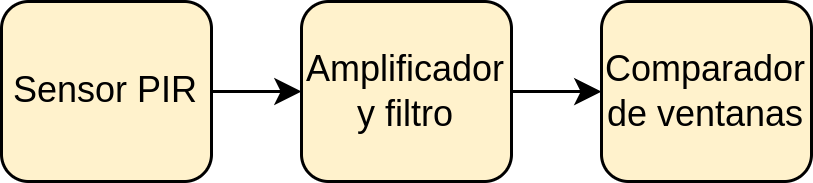
\includegraphics[scale=0.25]{./Figures/move_blocks.png}
	\caption{Diagrama en bloques del sensor de movimiento PIR.}
	\label{fig:move_blocks}
\end{figure}

\subsubsection{Sensor pasivo infrarojo}
El IRA-S230ST01 es un sensor PIR fabricado por la empresa Murata. Posee una alta sensibilidad y un rendimiento confiable gracias a la tecnología cerámica y la técnica de IC (\textit{Integrated Circuit}, Circuito Integrado) híbrida de Murata. Tiene además una sensibilidad mejorada a la interferencia de RF (\textit{Radio Frequency}, Radiofrecuencia). Sus aplicaciones más comunes incluyen sistemas de seguridad, aparatos de iluminación, electrodomésticos, entre otros \cite{pir_info}. En la figura \ref{fig:pir_photo} se puede observar una fotografía del IRA-S230ST01.

\vspace*{60 px}

\begin{figure}[h]
	\centering
	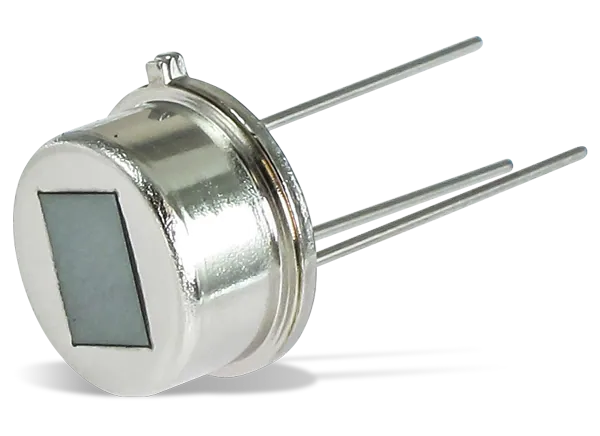
\includegraphics[scale=0.2]{./Figures/pir_photo.png}
	\caption{Fotografía del sensor IRA-S230ST01\protect\footnotemark.}
	\label{fig:pir_photo}
\end{figure}
\footnotetext{Imagen tomada de: \url{https://www.murata.com/en-sg/products/productdetail?partno=IRA-S230ST01}}

En la tabla \ref{tab:pir_specs} se detallan sus características técnicas más importantes

\begin{table}[h]
	\centering
	\caption[IRA-S230ST01 especificaciones]{Tabla de especificaciones del IRA-S230ST01 \cite{pir_info}}
	\begin{tabular}{lc}   
		\toprule
		\textbf{Característica} 	 & \textbf{Descripción}  \\
		\midrule
		Rango de temperatura & -40 \textcelsius  a 70 \textcelsius\\
		SNR & 40 dB \\
		Campo de vision & theta1=theta2=45 grados \\
		Electrodo & (2.0x1.0mm)x2 \\
		Responsividad & 4.6 mV \\
		Filtro óptico & 5 \textmu m paso alto \\
		Fuente de alimentacion & 2 V a 15 V \\
		\bottomrule
		\hline
	\end{tabular}
	\label{tab:pir_specs}
\end{table}

La elección del IRA-S230ST01 como sensor PIR responde a los siguientes criterios: \\
\begin{itemize}
	\item Marca: Murata es una marca muy reconocida en el mundo de los semiconductores y ofrece productos de muy alta calidad.
	\item Documentación: el IRA-S230ST01 cuenta con documentación muy clara sobre sus características técnicas.
\end{itemize}

\subsubsection{Amplificador operacional}
El TLV8544 es un amplificador operacional cuadruple de ultra bajo consumo energético de la empresa Texas Instruments, de costo optimizado para aplicaciones de detección en equipos inalámbricos y cableados de bajo consumo. El diseño del TLV8544 minimiza el consumo energético en dispositivos como sensores de movimiento para sistemas de seguridad, donde el tiempo de vida de la batería que los alimenta es crítico. Su uso más común es en configuraciones de amplificadores de transimpedancia con resistencias de \textit{feedback} en el orden de los Mega ohms. Adicionalmente, tiene protección contra EMI (\textit{Electromagnetic Interference}, Interferencia Electromagnética) que reduce la sensibilidad a las señales de RF no deseadas de fuentes como teléfonos móviles, Wi-Fi y transmisores de radio \cite{opamp_info}. En la figura \ref{fig:opamp_photo} se puede observar una fotografía del TLV8544 en un encapsulado TSSOP-14.

\vspace*{50 px}

\begin{figure}[h]
	\centering
	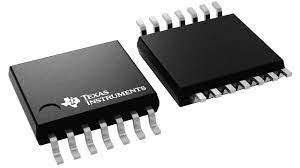
\includegraphics[scale=0.4]{./Figures/opamp_photo.jpeg}
	\caption{Fotografía del TLV8544 en un encapsulado TSSOP-14\protect\footnotemark.}
	\label{fig:opamp_photo}
\end{figure}
\footnotetext{Imagen tomada de: \url{https://www.ti.com/product/TLV8544}}

Las características técnicas más importantes del TLV8544 se presentan en la tabla \ref{tab:opamp_specs}.

\begin{table}[h]
	\centering
	\caption[TLV8544 especificaciones]{Tabla de especificaciones del TLV8544 \cite{opamp_info}}
	\begin{tabular}{lc}   
		\toprule
		\textbf{Característica} 	 & \textbf{Descripción}  \\
		\midrule
		Número de canales & 4 \\
		Fuente de alimentación & 1.7 V a 3.6 V \\
		Corriente de salida por canal & 30 mA \\
		Corriente de operación & 500 nA \\
		CMMR (\textit{Common Mode Rejection Ratio}, \\ Relación de Rechazo del Modo Común) & 90 dB \\
		Rango de temperatura & -40 \textcelsius  a 125 \textcelsius\\
		Corriente de polarización & 100 fA \\
		Ancho de banda de ganancia & 8 kHz \\
		\bottomrule
		\hline
	\end{tabular}
	\label{tab:opamp_specs}
\end{table}

Desde hace muchos años los amplificadores operacionales son dispositivos muy utilizados por su gran cantidad de aplicaciones, en el mercado existen una gran variedad de modelos y son fabricados por muchas empresas de semiconductores. Estos fueron los criterios de elección del TLV8544 para el presente trabajo:
\begin{itemize}
	\item Aplicación: por sus características técnicas, el TLV8544 está diseñado para ser parte de las etapas de amplificación y filtrado en el diseño de un sensor de movimiento PIR.
	\item Documentacion: Texas Instruments, además del correspondiente \textit{datasheet} del TLV8544, ofrece varios documentos técnicos con ejemplos de diseño para el TLV8544.
	\item Costo: es un dispositivo de precio muy razonable por todas las características que ofrece.
	\item Consumo energético: con sus 500 nA de corriente de funcionamiento por canal, el TLV8544 es una opción ideal para aplicaciones que requieran el uso de baterías.
\end{itemize}

\subsection{Cámara}
Otro de los componentes principales del sistema es la cámara, que permite obtener imágenes en un formato digital que posteriormente deben ser procesadas por los algoritmos de DL. Para este trabajo se utilizó el módulo ESP-LyraP-CAM. Este módulo integra un CCM (\textit{Compact Camera Module}, Módulo de Cámara Compacto) con un sensor OV2640 en conjunto con dos reguladores de tensión para su correcto funcionamiento. En la figura \ref{fig:camera_comp} se puede observar unas fotografías del módulo ESP-LyraP-CAM y sus componentes.

\begin{figure}[h]
	\centering
	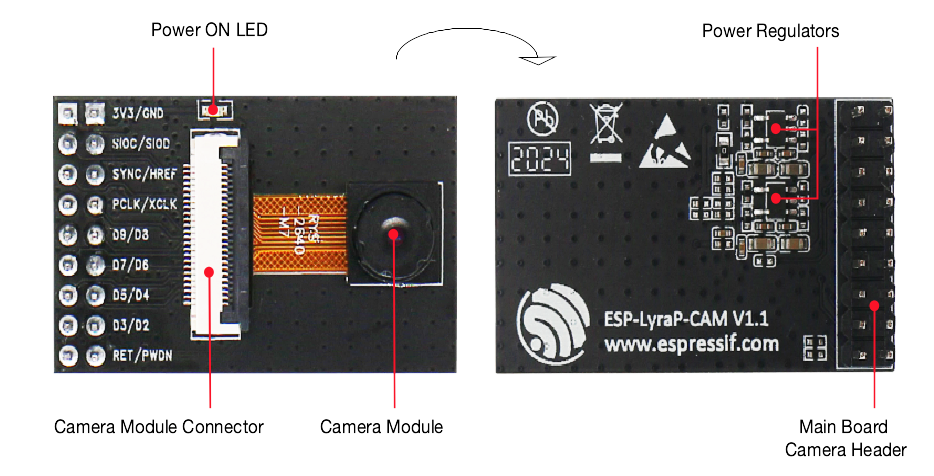
\includegraphics[scale=0.6]{./Figures/camera_blocks.png}
	\caption{Componentes del módulo ESP-LyraP-CAM\protect\footnotemark.}
	\label{fig:camera_comp}
\end{figure}
\footnotetext{Imagen tomada de: \url{https://docs.espressif.com/projects/esp-idf/en/latest/esp32s2/hw-reference/esp32s2/user-guide-esp-lyrap-cam-v1.1.html}}

El OV2640 de la empresa OmniVision es un sensor CMOS (\textit{Complementary Metal-Oxide-Semiconductor}, Semiconductor de Óxido de Metal Complementario) de 2 MP, cuenta con una interfaz de comunicación compatible con DVP  (\textit{Digital Video Port}, Puerto de Video Digital), soporta codificación JPEG (\textit{Joint Photographic Experts Group}, Grupo Unido de Expertos en Fotografía) y es de bajo consumo energético. En la tabla \ref{tab:ov2640_specs} se muestran las características técnicas más importantes del OV2640.

\begin{table}[h]
	\centering
	\caption[OV2640 especificaciones]{Tabla de especificaciones del OV2640 \cite{camera_info}}
	\begin{tabular}{lc}   
		\toprule
		\textbf{Característica} 	 & \textbf{Descripción}  \\
		\midrule
		Tamaño de matriz & 1600x1200 (UXGA) \\		
		Fuente de alimentación & \begin{tabular}{@{}c@{}} \textit{Core}: 1.3 V ± 5\% \\ \textit{Analog} 2.5 ~ 3.0 V \\ I/O: 1.7 V - 3.3 V\end{tabular} \\
		Consumo energético & \begin{tabular}{@{}c@{}} \textit{Free running}: 125 mW \\ \textit{Standby}: 600 \textmu A \end{tabular} \\
		Formato de imagen del sensor & 1/4'' \\
		Tasa de transferencia maxima & \begin{tabular}{@{}c@{}} 1600×1200 a 15 fps \\ SVGA a 30 fps \\ CIF a 60 fps \end{tabular} \\
		Sensibilidad & 0.6 / Lux-sec \\
		SNR & 40 dB \\
		Rango dinámico & 50 dB \\
		Tamano de pixel & x2.2x2.2 \textmu m \\
		Formato de salida & YUV/RGB/MJPEG \\
		\bottomrule
		\hline
	\end{tabular}
	\label{tab:ov2640_specs}
\end{table}

Los criterios para utilizar este módulo como cámara del sistema son los siguientes:
\begin{itemize}
	\item Costo: los módulos con el sensor OV2640 tienen un costo muy reducido en comparación con otros disponibles en el mercado.
	\item Bajo consumo energético: como se mostró en la tabla \ref{tab:ov2640_specs} el consumo energético del módulo en modo \textit{standby} es lo suficientemente bajo como para funcionar alimentado por baterías.
	\item Disponibilidad de código: al ser un módulo que ya lleva mucho tiempo en el mercado existen muchas bibliotecas de código para utilizarlo, lo que simplifica en gran medida el tiempo de desarrollo de \textit{firmware}.
\end{itemize}

%----------------------------------------------------------------------------------------
\section{Redes Convolucionales en Cascada Multitarea}
MTCNN (\textit{Multi-task Cascaded Convolutional Networks}, Redes Convolucionales en Cascada Multitarea) es un \textit{framework} basado el el \textit{paper} ``Joint Face Detection and Alignment using Multi-task Cascaded Convolutional Networks`` de Kaipeng Zhang, Zhanpeng Zhang, Zhifeng Li y Yu Qiao \cite{mtcnn_info}, está desarrollado para integrar las tareas de detección facial y alineamiento facial con ayuda de CNNs en cascada mediante aprendizaje multitarea. El proceso consta de tres etapas de CNNs que puede detectar rostros humanos, sus posiciones y las posiciones de sus rasgos faciales (nariz, ojos y boca). En la figura \ref{fig:mtcnn_pipe} se muestra el \textit{pipeline} utilizado en MTCNN.

\begin{figure}[h]
	\centering
	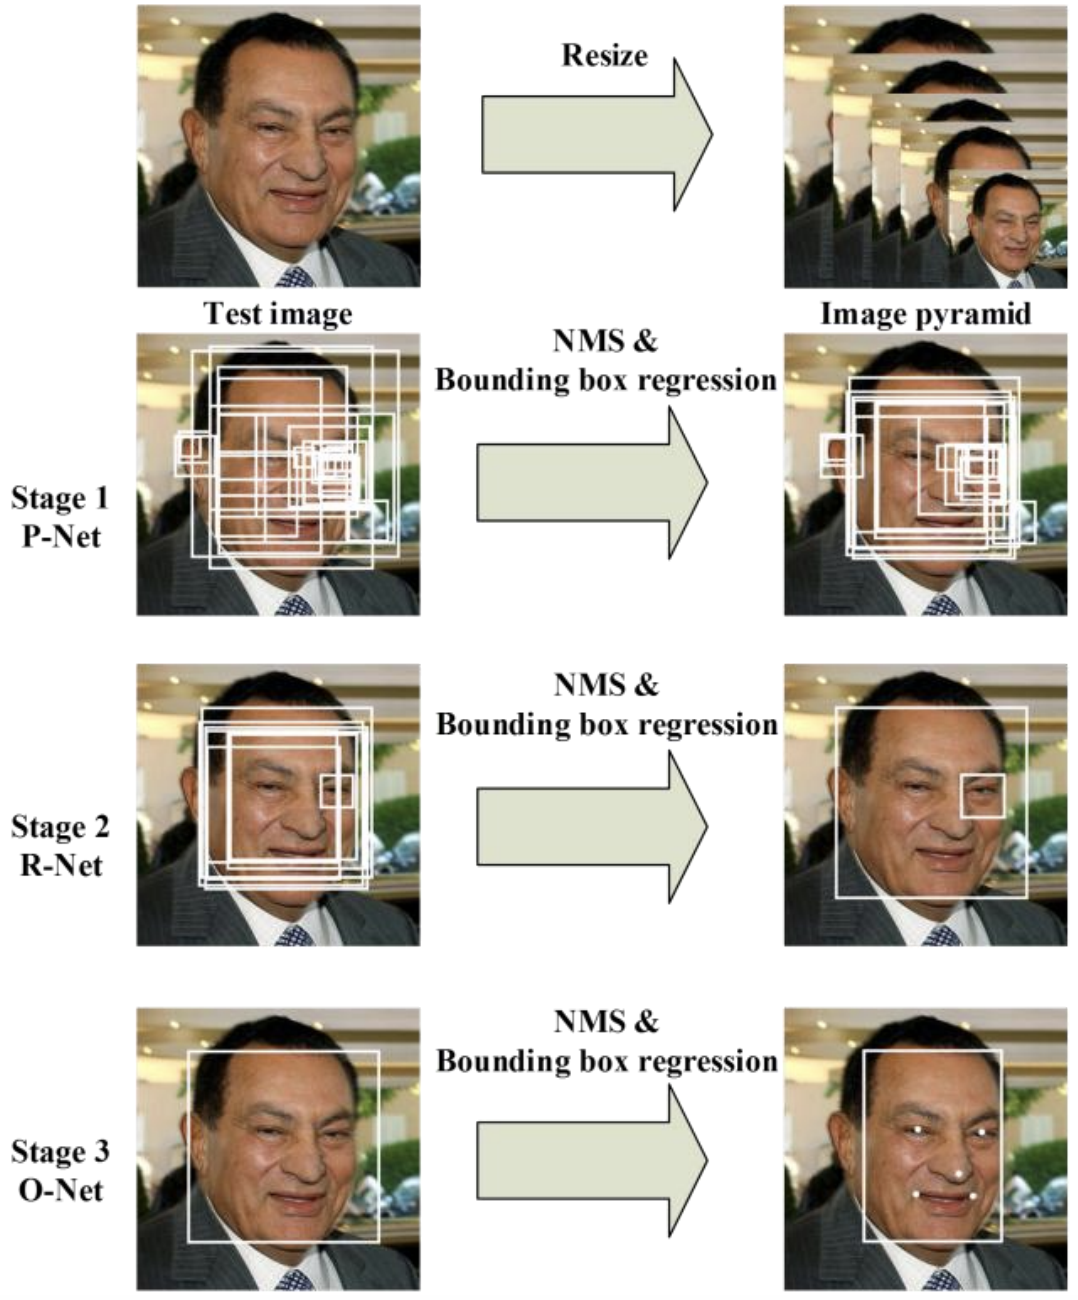
\includegraphics[scale=0.5]{./Figures/mtcnn_pipe.png}
	\caption{\textit{Pipeline} de MTCNN \cite{mtcnn_info}.}
	\label{fig:mtcnn_pipe}
\end{figure}

\subsection{Red de propuestas}
También conocida como P-Net (\textit{Proposal Network}, Red Propositiva), esta etapa está compuesta de una FCN (\textit{Fully Convolutional Network}, Red Totalmente Convolucional). La diferencia entre una FCN y una CNN es que la FCN no utiliza una capa FC como parte de su arquitectura. Tiene la función de obtener ventanas candidatas y sus vectores de regresión de \textit{bounding box} a partir de varias escalas de la imagen original. La regresión de \textit{bounding box} es una técnica para predecir la localización de un cuadro delimitador en el que se encuentra el objeto que quiere ser detectado, en este caso rostros humanos. Una vez que se obtienen estos vectores, se realiza una operación conocida como NMS (\textit{Non Max Suppression}, Supresión no Máxima) para combinar las regiones superpuestas entre sí. Finalmente las ventanas candidatas resultantes pasan a la siguiente etapa. En la figura \ref{fig:mtcnn_pnet} se muestra la arquitectura de P-Net.

\begin{figure}[h]
	\centering
	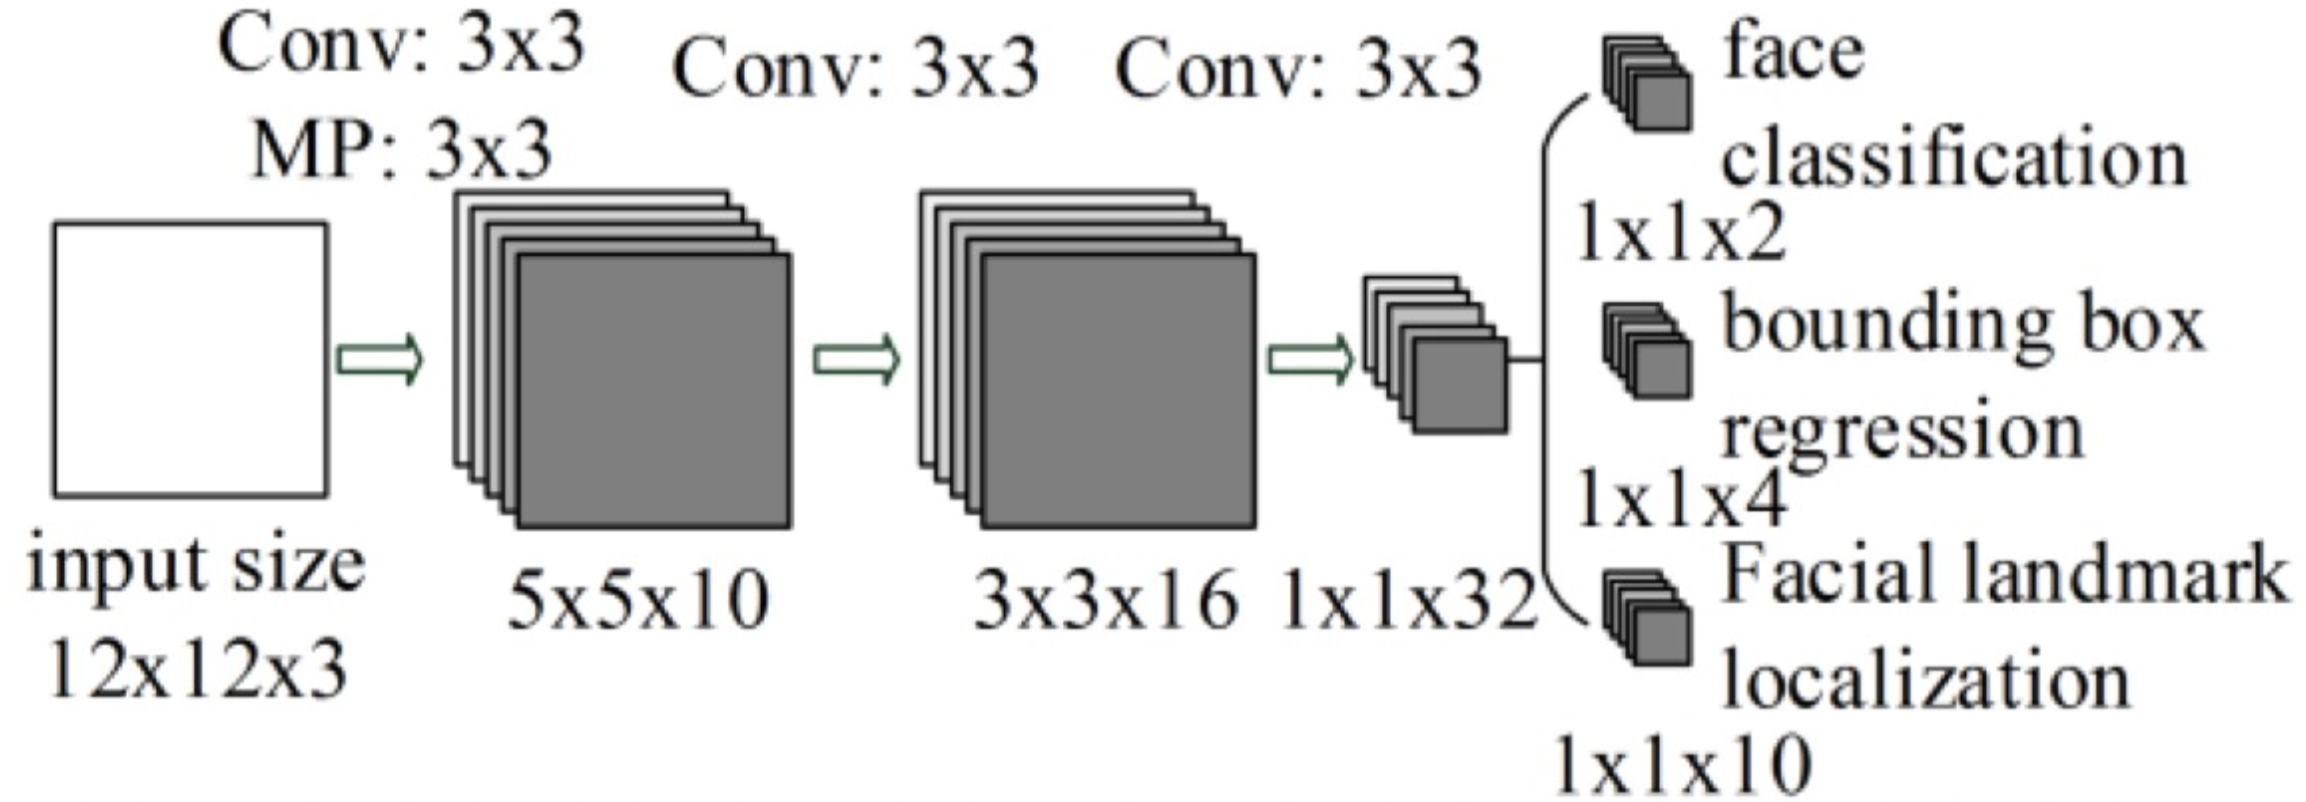
\includegraphics[scale=0.25]{./Figures/mtcnn_pnet.png}
	\caption{Arquitectura de P-Net \cite{mtcnn_info}.}
	\label{fig:mtcnn_pnet}
\end{figure}
	
\subsection{Red de refinamiento}
Esta es una CNN denominada R-Net (\textit{Refine Network}, Red de Refinamiento). Los candidatos provenientes de P-Net son la entrada de esta red. La arquitectura de R-Net reduce aún más el número de candidatos, realiza la calibración con regresión de \textit{bounding box} y emplea NMS para fusionar candidatos superpuestos. Para cada candidato de entrada, R-Net obtiene la probabilidad de si es un rostro o no, un vector de 4 elementos que es el \textit{bounding box} y un vector de 10 elementos que representan la localización de rasgos faciales. En la figura \ref{fig:mtcnn_rnet} se muestra la arquitectura de R-Net.

\begin{figure}[h]
	\centering
	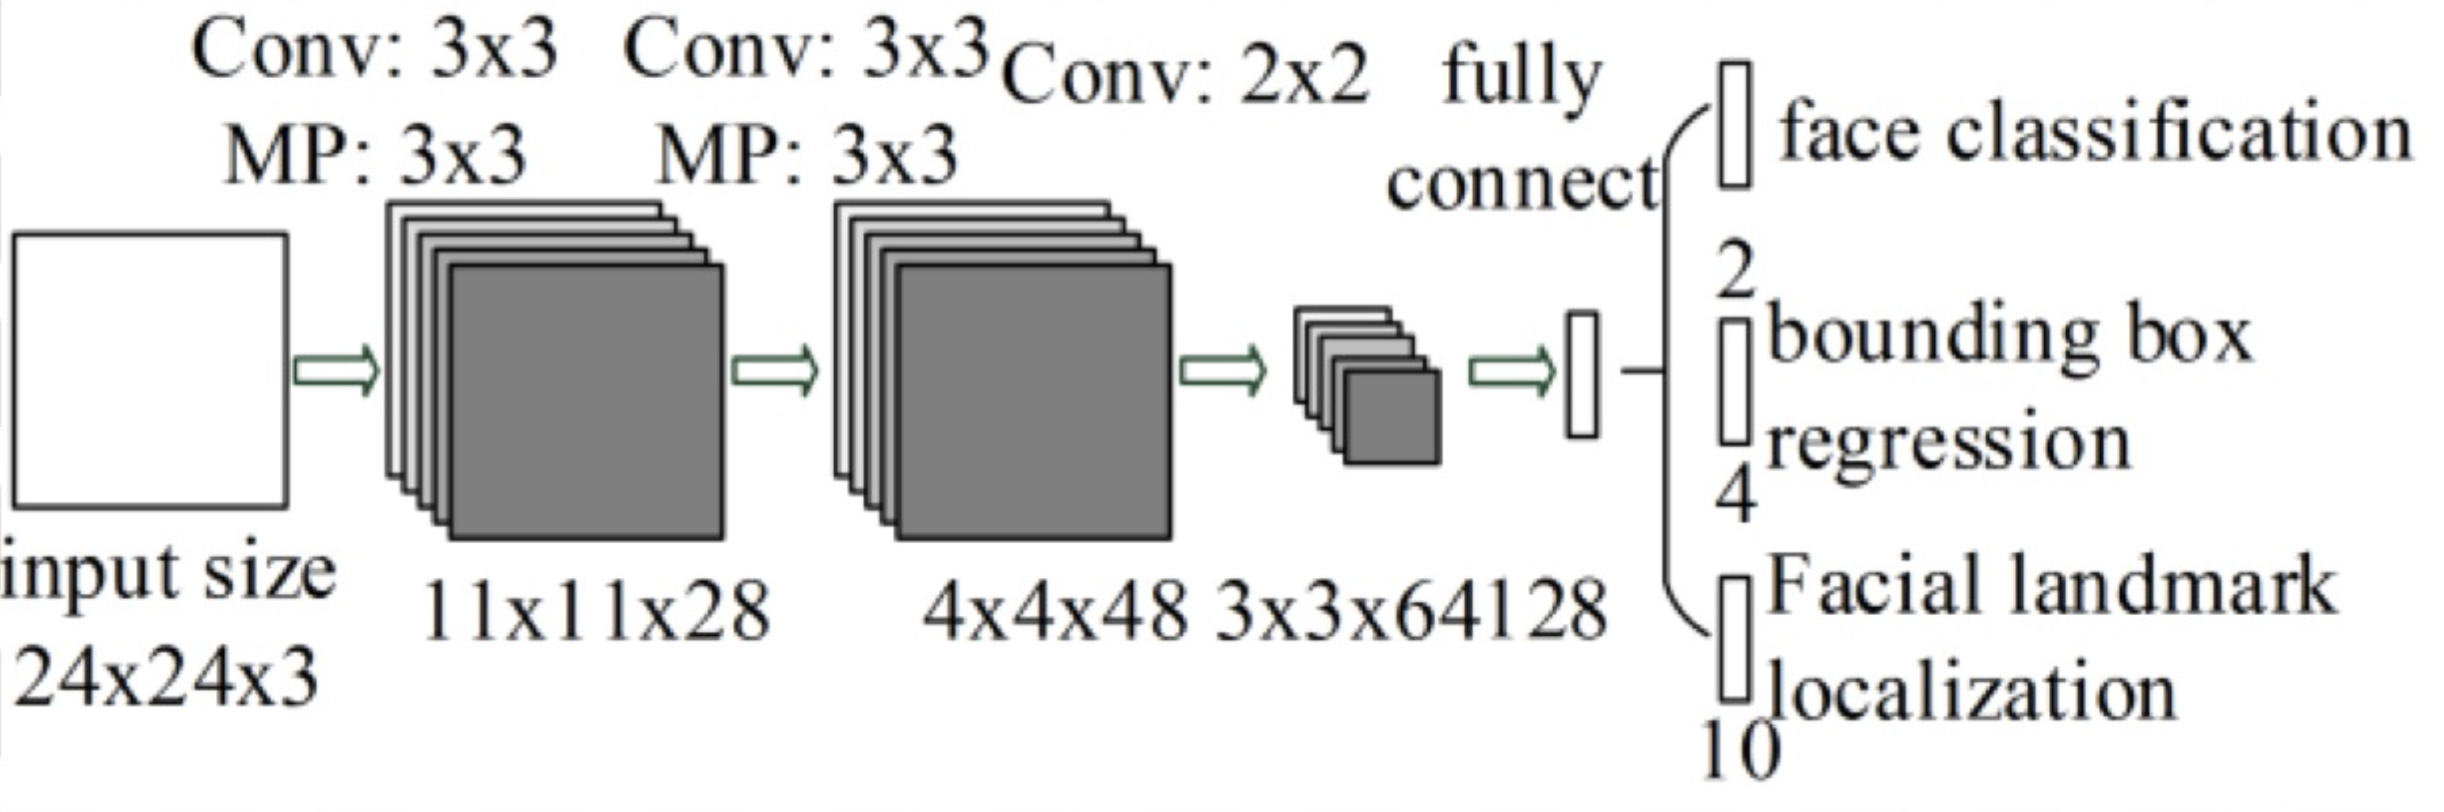
\includegraphics[scale=0.25]{./Figures/mtcnn_rnet.png}
	\caption{Arquitectura de R-Net \cite{mtcnn_info}.}
	\label{fig:mtcnn_rnet}
\end{figure}

\subsection{Red de salida}
Conocida como O-Net (\textit{Output Network}, Red de Salida), es muy similar a R-Net, pero está enfocada a describir el rostro con más detalle y generar las cinco localizaciones para ojos, boca y nariz. Su arquitectura se muestra en la figura \ref{fig:mtcnn_onet}.

\begin{figure}[h]
	\centering
	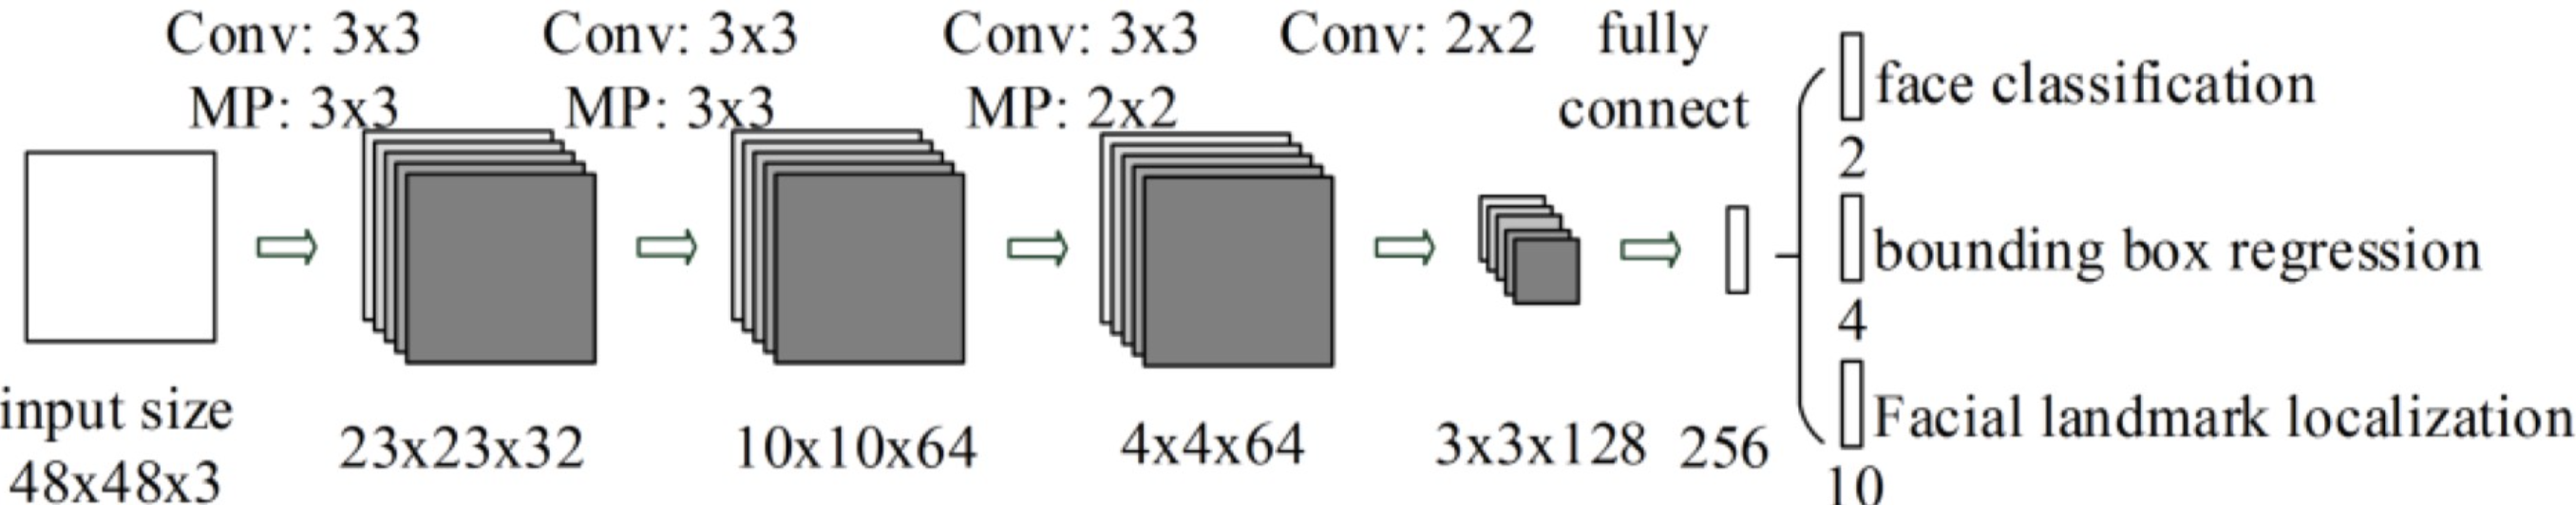
\includegraphics[scale=0.3]{./Figures/mtcnn_onet.png}
	\caption{Arquitectura de O-Net \cite{mtcnn_info}.}
	\label{fig:mtcnn_onet}
\end{figure}

\subsection{Tareas}
Como se explicó en los puntos anteriores, MTCNN se compone de tres etapas que filtran ventanas candidatas y con la ayuda de NMS y calibración con los vectores de regresión de \textit{bounding box}, se detectan rostros y sus rasgos. Entonces, el propósito de MTCNN es cumplir con las siguientes tareas:
\begin{itemize}
	\item Clasificación rostro/no rostro: este es un problema de clasificación binaria que utiliza una función de pérdida de entropía cruzada.
	\item Regresión de \textit{bounding box}: el objetivo de aprendizaje es un problema de regresión. Para cada candidato, se calcula el \textit{offset} entre el candidato y el \textit{ground truth} [ref] más cercano. La función de pérdida Euclidiana es utilizada para esta tarea.
	\item Localización de rasgos faciales:es formulada como un problema de regresión en el que la función de perdida es la distancia Euclidiana.
\end{itemize}

%----------------------------------------------------------------------------------------
\section{Biblioteca TensorFlow}
TensorFlow es una plataforma de código abierto para ML. Tiene un ecosistema completo y flexible de herramientas, bibliotecas y recursos comunitarios que permite a los desarrolladores crear e implementar fácilmente aplicaciones basadas en ML. Fue originalmente desarrollado por investigadores e ingenieros que trabajaban en el equipo Google Brain dentro de la organización de investigación de inteligencia artificial de Google y la versión inicial fue lanzada en 2015 bajo la licencia Apacha License 2.0 \cite{tf_info}. TensorFlow proporciona APIs estables y oficiales para Python y C++, aunque también existen APIs para otros lenguajes de programación que no están garantizadas de manera oficial.

Sus características principales son:
\begin{itemize}
	\item Autodiferenciación: es el proceso de cálculo automático del vector gradiente de un modelo respecto a cada uno de sus parámetros.
	Ejecución ansiosa: significa que las operaciones se evalúan de manera inmediata en lugar de agregarse a un gráfico computacional que se ejecuta más tarde.
	\item Distribuido: TensorFlow proporciona una API para distribuir el cómputo en múltiples dispositivos tanto para ejecución ansiosa como para gráficos computacionales.
	\item Funciones de pérdida: TensorFlow proporciona un conjunto de funciones de pérdida, también conocidas como funciones de costo.
	\item Métricas: TensorFlow brinda acceso a un API de métricas de uso común que se utilizan para evaluar el rendimiento de los modelos de ML.
	Optimizadores: TensorFlow ofrece un conjunto de optimizadores para entrenar redes neuronales, algunos son ADAM, ADAGRAD y SGD (\textit{Stochastic Gradient Descent}, Descenso de Gradiente Estocástico).
\end{itemize}

Para el desarrollo de aplicaciones de ML existen varias otras bibliotecas, algunas de las más populares son: PyTorch, Caffe Computer Vision Library, Deeplearning, Neuroph, OpenNN, Theano, Torch y MXNet. Los criterios de elección de TensorFlow en este trabajo sobre las anteriores bibliotecas citadas fueron:
\begin{itemize}
	\item Experiencia: este fue el criterio más fuerte en elección de TensorFLow como \textit{framework} para el desarrollo de modelos de ML. El autor de este trabajo ya poseía experiencia trabajando con TensorFlow.
	\item Documentación: TensorFlow tiene mucha documentación oficial sobre su API y una gran variedad de tutoriales de uso.
	\item Herramientas para cuantización: TensorFlow cuenta con herramientas de cuantización de datos para optimizar el tamaño y tiempos de ejecución de modelos de ML.
\end{itemize}

%----------------------------------------------------------------------------------------
\section{Servicios Web de Amazon}
Más conocido como AWS (\textit{Amazon Web Services}, Servicio Web de Amazon) por sus siglas en inglés, es una plataforma de \textit{cloud computing} provista por Amazon que incluye una combinación de IaaS, PaaS y SaaS. Los servicios de AWS pueden ofrecer herramientas de poder cómputo, almacenamiento de datos y servicios de entrega de contenido \cite{aws_info}.

AWS está dividido en distintos tipos de servicios que pueden ser configurados según las necesidades de cada usuario. Estos servicios pueden dividirse en las siguientes categorías: computación, almacenamiento, bases de datos, administración de datos, migración, redes, herramientas de desarrollo, monitoreo, administración de \textit{big data}, analíticas, AI, desarrollo móvil, mensajería y notificaciones.

De toda la extensa cantidad de servicios que ofrece AWS, para este trabajo se necesitaron sólo los siguientes: IoT Core y Amazon Timestream.

\subsection{Servicio IoT Core}
Proporciona los servicios en la nube necesarios para conectar dispositivos IoT entre sí y a los otros servicios de AWS \cite{iot_info}. AWS IoT proporciona software que puede ayudar a integrar dispositivos IoT en soluciones basadas en las herramientas de AWS. En la figura \ref{fig:aws_iot} se puede observar un diagrama de interconexión de dispositivos IoT y los servicios de AWS mediante IoT Core.


\begin{figure}[h]
	\centering
	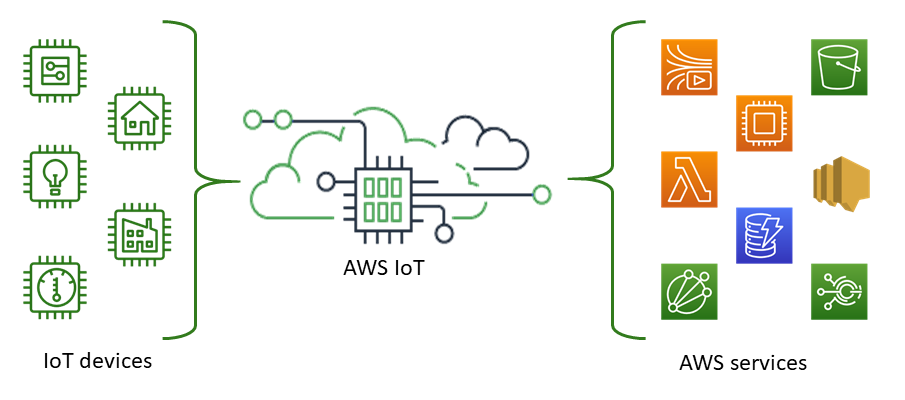
\includegraphics[scale=0.5]{./Figures/aws_iot.png}
	\caption{Diagrama de conexión entre dispositivos IoT y AWS\protect\footnotemark.}
	\label{fig:aws_iot}
\end{figure}
\footnotetext{Imagen tomada de: \url{https://docs.aws.amazon.com/iot/latest/developerguide/what-is-aws-iot.html}}

IoT Core permite seleccionar las tecnologías más adecuadas y actualizadas para interconectar dispositivos IoT. Los protocolos de comunicación soportados son: MQTT (\textit{Message Queuing and Telemetry Transport}, Cola de Mensajes y Transporte de Telemetría), MQTT sobre WSS (\textit{Websocket Secure}, Websocket Seguro), HTTPS (\textit{Hypertext Transfer Protocol Secure}, Protocolo de Transferencia de Hipertexto Seguro) y LoRaWAN.

El \textit{broker} de IoT Core admite dispositivos y clientes que utilizan MQTT y MQTT sobre WSS para publicar y suscribirse a algún tópico. También es compatible con dispositivos y clientes que utilizan HTTPS para publicar mensajes.

\subsection{Servicio TimeStream}
TimeStream es una base de datos de series temporales rápida, escalable y totalmente administrada, que facilita el almacenamiento y el análisis de billones de datos de series temporales al día. Timestream ahorra tiempos y costos con su capacidad de administrar los ciclos de vida de los datos de series temporales, donde mantiene los datos recientes en la memoria y mueve los datos históricos a un nivel de almacenamiento optimizado según las políticas definidas previamente por el usuario. El motor de consultas de Timestream permite acceder y analizar datos recientes e históricos al mismo tiempo. No necesita servidor y su tamaño se acomoda automáticamente para ajustar la capacidad y el rendimiento requeridos \cite{timestream_info}.

Los beneficios más notables que ofrece Amazon Timestream son:
\begin{itemize}
	\item Sin servidor con escalado automático: a medida que cambian las necesidades de la aplicación, Timestream escala automáticamente para ajustar la capacidad.
	\item Administración de los ciclos de vida de los datos: ofrece ofrece niveles de almacenamiento, con un almacenamiento de memoria para datos recientes y un almacenamiento magnético para datos históricos. Timestream automatiza el proceso de transferencia entre ambos almacenamientos.
	\item Acceso simplificado a los datos: el motor de consultas de Timestream permite acceder a los datos de forma transparente, sin la necesidad de especificar el nivel de almacenamiento.
	\item Diseñado para series temporales: puede analizar datos de series de tiempo con SQL, con funciones integradas de series de de tiempo para suavizar, aproximar e interpolar.
	\item Siempre cifrado: garantiza que los datos de series de tiempo siempre están cifrados. Timestream permite especificar una clave administrada para encriptar datos en el almacenamiento magnético.
	
\end{itemize}

%----------------------------------------------------------------------------------------
\section{Plataforma Grafana}
Es una aplicación web multiplataforma de análisis y visualización interactiva. Proporciona tablas, gráficos y alertas a través de la web cuando se conecta a alguna fuente de datos compatible. Los usuarios pueden crear \textit{dashboards} de monitoreo de datos complejos con ayuda de generadores de consultas interactivos \cite{grafana_info}.

Como herramienta de visualización, Grafana es muy popular gracias a las siguientes características:
\begin{itemize}
	\item Se conecta a muchas fuentes de datos populares como Graphite, Prometheus, Influxdb, ElasticSearch, MySQL, PostgreSQL, entre otros.
	\item Es de código abierto y distribuida bajo la licencia  AGPL-3.0, que permite desarrollar complementos desde cero para integrar con otras fuentes de datos.
	\item Ayuda a estudiar, analizar y monitorear datos durante un periodo de tiempo configurable por el usuario.
	\item Puede ser implementado localmente por organizaciones que quieran mantener sus datos confidenciales sin acceso a internet.
	\item Se pueden configurar alertas que se envían por otros medios de comunicación bajo ciertas condiciones pre establecidas.
\end{itemize}




